\documentclass[12pt]{extarticle}
\usepackage{lmodern} % Required for inserting images
\usepackage{graphicx} % Required for inserting images
\usepackage{amsmath}
\usepackage{amssymb}
\usepackage{amsfonts}
\usepackage{float}

\title{Statistics For Data Science}
\author{Akash Tesla}
\date{July 2025}

\begin{document}
\tableofcontents
\newpage
\maketitle
\section{Basic Terminologies}

\subsection{Population}
An entire set of items you want to study 

\subsection{Sample} 
A subset of population used to estimate statistical behavior of the whole population 

\subsection{Histogram}
A histogram is a graphical representation of numerical data that groups the data into bins and displays the frequency of data points within each bin as bars

\begin{figure}[H]
    \centering
    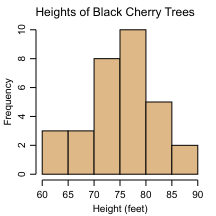
\includegraphics[width=0.5\linewidth]{images/histogram_example.png}
    \caption{Example of a Histogram}
    \label{fig:1}
\end{figure}


\section{Law of large numbers}
As the number of trials (or samples) increases, the sample average (or empirical mean) will converge to the expected value (or population mean).
\subsubsection{Weak Law of large numbers}
The weak law states that the sample average of a sequence of independent identically distributed(i.i.d.) random variables converges in probability to the expected value as the number of samples goes to infinity
$$\bar{X_n} = \frac{1}{n}\sum_{i=1}^{n}X_i \xrightarrow{p} \mu \quad as \ n \to \infty $$
which means, 
$$\forall \varepsilon>0, \lim_{n \to \infty}^n \mathbf{p}(|\bar{X}_n-\mu| > \varepsilon) = 0 $$
\subsubsection{Strong Law of large numbers}
The strong law states that the sample average of a sequence of i.i.d. random variables converges almost surely to the expected value as the number of samples goes to infinity 

$$\bar{X}_n = \frac{1}{n} \sum_{i=1}^n X_i \xrightarrow{a.s.} \mu \quad as\ n \to \infty$$
Which means, 
$$ \mathrm{P}(\lim_{n \to \infty} \bar{X}_n = \mu ) = 1 $$

\section{Central-Limit Theorem}

\section{Types of Data}
\subsection{Qualitative Data}
Describes Qualities, Charesteristics , or categories
\subsubsection{Nominal}
Pure categories without order, 
Example: blood type(A,B,AB,O), brand names
\subsubsection{Ordinal}
Categories with meaningfull order,
Examples: Rank, Survey rating
\subsection{Quantitative Data}
Measureable quantities, Number have meaningfull terms in terms of magnitude
\subsubsection{Discrete}
Countable values, no in-betweens. 
Examples: number of cars
\subsubsection{Continuous}
Countinous measurements; can take any value within a range, 
Examples: Height, weight, temperature

\section{Measure of Central Tendency} 

\subsection{Mean/Expected Value} 
Average of all data points, sensitive to outliers since a single large outlier could easily skew mean 

$$ \mu = \frac{\sum x_i}{n} $$ 

\subsection{Median}
The middle data point when data are stored, robust to outliers 

\subsection{Mode}
The most frequent data point of the dataset  

\section{Measure of Spread}
Range: Difference between minimum value and maximum value 

$$ Range = x_{max} - x_{min} $$ 

\subsection{Variance}
Average squared deviation, Variance represents Expected variance between mean and data points,
It's basically MSE of a model that just predicts mean, that kinda gives an intutitive 
understanding of how it measures spread

$$\sigma^2 = E[(X - \mu)^2]$$
$$\sigma^2 = E[(X - E[X])^2]$$
$$\sigma^2 = E[X^2]-(E[X])^2$$
$$ \sigma^2 = \frac{\sum (x_i - \mu)^2}{n} (Population) $$ 
$$ s^2 = \frac{\sum( \bar{x_i} - \mu)^2}{n-1} (Sample)  $$ 

\subsection{Standard Deviation}
Root of Variance, 
RMSE of a model that just predicts mean, 
standard deviation gives in intrepretable terms like RMSE

$$ \sigma = \sqrt{\sigma^2} $$
\subsection{Inter Quartile Range(IQR)}
Difference between 75th Percentile/3rd Quartile and 25th Percentile/1st Quartile, it is used for outlier detection 
$$IQR = Q_3 - Q_1$$ 
We calculate lower bounds and upper bounds to detect the outliers
$$ \text{lower bound}= Q1-1.5 \times IQR$$
$$ \text{upper bound}= Q3+1.5 \times IQR$$
the data points which values outside of the bounds is considered to be outliers, for more extreme detection \(3 \times IQR\) is also used

\section{Probability Distributions}

\subsection{Discrete Distributions}
A discrete probability distribution describes the probability of occurrence of each value of a discrete random variable
\begin{itemize}
    \item Discrete random variable: Countable values like 1,2,3
    \item Each individual value has an associated probability 
    \item The sum of probabilities for all possible values is 1
    $$ \sum_i \mathrm{P}(X=x_i)=1$$
\end{itemize}

\subsection{Continuous Distributions}

\section{Discrete Probability Distributions}
\subsection{Benoulli Distribution}
The benouli distribution is a discrete probability distribution for a random variable which takes only two possibilities, Sucess or a failure 
\subsubsection{Probability Mass Function(PMF)}
$$
P(X=x) = 
\begin{cases}
    p & \text{if x=1} \\
    1-p & \text{if x=0} \\
    0 & \text{Otherwise}
\end{cases}
$$
Also written as 
$$ \mathrm{P}(X=x) = p^x(1-p)^{1-x}, \quad \text{for x }\epsilon \ \{0,1\}$$

\subsubsection{Statistical Parameters}
\textbf{Mean}\\
Mean is the expected value over many repetitions of the same single-trial experiment,
thus it would be p since, p is probability of 1 appearing and (1-p) is probability of 0 appearing
$$\mu = 1 \times (p)+0 \times (1-p)$$
$$\mu = p$$
\textbf{Variance}\\
Variance can be defined as \( \sigma^2 = E(X^2) - (E(x))^2\), Refer Variance chapter. 
For Bernoulli distribution, \(E(X^2) = p, E(X) = p\), substituting we get
$$\sigma^2 = p - p^2$$
$$\sigma^2 = p(1-p)$$
\textbf{Mode}\\
Mode for Bernoulli would what ever the outcome which is more favored, which can be defined as  
$$
Mode = 
\begin{cases}
    1 & \text{If \(p > 0.5 \)}  \\
    0 & \text{If \(p < 0.5\)}
\end{cases}
$$
\subsubsection{Examples}
\begin{itemize}
    \item Will it rain tomorrow?
    \item Will this patient recover?
    \item Will this product be defective?
\end{itemize}

\begin{figure}[H]
    \centering
    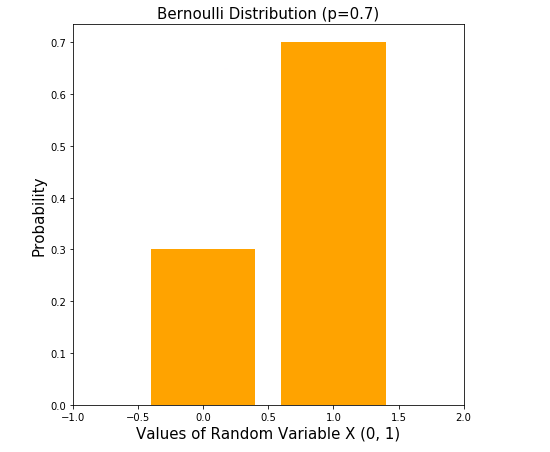
\includegraphics[width=0.5\linewidth]{images/bernoulli_example.png}
    \caption{Example of a Bernoulli Distribution}
    \label{fig:enter-label}
\end{figure}

\subsection{Binomial}
Binomial Distribution is a discrete probability distribution that models the probability of obtaining a specific number of successes
in a fixed number of independent trials(n), these independent trials are just Bernoulli trials, you could see the similarity between
them in statistical parameters

\subsubsection{Probability Mass Function(PMF)}

$$ P(X=x) = nCx \times p^x \times (1-p)^{(n-x)} $$
where,\\
n - no of trials,\\ 
p - probability of success\\
x - number of success\\

\subsubsection{Statistical Parameters}
\textbf{Mean}\\
Mean represents Average number of success from your trails which would be number of trials (n) times probability of success (p)
$$ \mu = n \times p $$
\textbf{Variance}\\
Variance represents Expected variance between mean and data points,
$$ \sigma^2 = n \times p \times (1-p) $$
\textbf{Mode}\\
$$ Mode = 
\begin{cases}
  \text{floor(n+1)p)} & \text{if (n+1)p is not an Integer} \\
  \text{floor((n+1)p), floor((n+1)(1-p))} & \text{if (n+1)p is an Integer} \\
\end{cases}$$ \\
$$ \text{Mode(if p = 0.5)} = 
\begin{cases}
  \frac{n}{2} & \text{if (n+1)p is not an Integer} \\
  \frac{(n-1)}{2},\frac{(n+1)}{2} & \text{if (n+1)p is an Integer} \\
\end{cases}
$$
\subsubsection{Examples}
\begin{itemize}
    \item How many patients will recover out of 50?
    \item How many rainy days this month?
    \item How many defective products in a batch of 1000?
\end{itemize}

\subsection{Negative-Binomial}
\subsection{Multinomial}
\subsection{Geometric}
\subsection{Hypergeometric}
\subsection{Poisson}
\subsection{Discrete Uniform}



\subsubsection{Use cases}
\begin{itemize}
    \item When there is only one trial
    \item When the outcome is binary True/False Yes/No 
\end{itemize}




\section{Shape fo the Distributions}
\subsection{Skewness} 
Measure of Asymmetry  
\subsubsection{Right-skewed} 
tail on the right (\(mean > median\)) 

\subsubsection{Left-skewed}
tail on the left (\(mean < median\))

\section{Evaluation Metrics for Regression}

\subsection{Mean Absolute Error}  

$$MAE = \frac{1}{n}\sum{|y_i - \hat{y_i}|}$$ 
\begin{itemize}
    \item Robust to outliers, treats all errors equally doesn’t square the errors like RMSE,MSE..etc 
    \item It’s used when your model can tolerate moderate outliers  
    \item Interpretability - Has same unit as the thing you are predicting/easy to understand 
    \item Gives out constant gradient (bad for gradient based loss function) 
\end{itemize}
 
\subsubsection{Gradient of MAE} 
$$
\frac{d}{d\hat{y}}|y - \hat{y}| = 
\begin{cases} 
+1 & \text{if }  \hat{y} < y \\ 
-1 & \text{if }  \hat{y} > y \\ 
\text{undefined} & \text{if } \hat{y} = y 
\end{cases} 
$$
As you can see no matter how far the error is from true value it always gives a constant gradient as it treats every error as same
stics
\subsection{Mean Squared Error}
$$MSE = \frac{1}{n}\sum{(y_i - \hat{y_i})^2}$$ 
\begin{itemize}
    \item Penalizes large errors/outliers 
    \item Gives out strong gradient signals  
\end{itemize}
\subsubsection{Gradient of MSE}
$$\frac{d MSE}{d\hat{y}} = -\frac{2}{n}(y-\hat{y})$$
It points in the direction of the error, and it grows linearly with size of the error
Larger the gradient, when prediction are more wrong \(\longrightarrow\) model adjusts faster


\subsection{Root Mean Squared Error(RMSE)}  
$$RMSE = \sqrt{MSE}$$ 
\begin{itemize}
    \item It combines interpretability of MAE and sensitive to errors of MSE
    \item It has smooth gradient curves just like MSE, and it's preferred for gradient descent 
\end{itemize}

\subsubsection{Gradient of RMSE}
$$ \frac{d RMSE}{\hat{y_i}} = \frac{1}{n \times RMSE} (\hat{y_i}-y_i)$$
\begin{enumerate}
    \item The gradient strength changes with RMSE, if your RMSE is very large the gradient becomes small, and if your RMSE is very small the gradient becomes large.
    \item It makes RMSE a Non-constantly scaled loss
    \item MSE is preferred over RMSE in training, but RMSE is preferred while reporting for interpretability  
\end{enumerate}

\subsection{R-Square(\(R^2\))}
\(R^2\) is the coefficient of determination. it tells how well your regression model 
explains the variation in the dependent variable(Y) using independent variables(X)
$$R^2 = 1-\frac{SS_{res}}{SS_{tot}}$$
where,
\begin{itemize}
    \item \(SS_{res} = \sum(y_i - \hat{y_i})^2 \to\) Residual sum of squares(error)/MSE
    \item \( SS_{tot} = \sum(y_i - \bar{y_i})^2 \to\) Total sum of squares (total variability)
\end{itemize}
$$R^2 = 1-\frac{ \sum(y_i - \hat{y_i})^2 }{ \sum(y_i - \bar{y_i})^2} $$
Or, it can also be written more intuitively as 
$$ R^2 = 1 - \frac{MSE}{\sigma^2} $$

\begin{itemize}
    \item Let us understand the formula (1-) operator just switches from maximizing to minimizing
so you can ignore that. \\
    \item \(\frac{MSE}{\sigma^2}\) Explains how well our model performs to a model that 
just predicts mean everytime, so if the ratio is 1, then our model is same as the dumb model,
we have to reduce the ratio but the world likes "more the better" approach 
add (1-) operator we have to maximize the error and it's called as \(R^2\) 
\item \(R^2\) ranges from \((-\infty,1]\)
\end{itemize}

\subsection{Adjusted \(R^2\)}
$$ R^2_{adj} = 1 - \left(\frac{(1-R^2)(n-1)}{n-k-1}\right) $$
The above mentioned is textbook formula but we use our simplified 
representation for \(R^2\)
$$ R^2 = 1 - \frac{MSE}{\sigma^2} $$
so, \(R^2_{adj}\) would be
$$ R^2_{adj} = 1 - \frac{MSE_{adj}}{\sigma^2_{adj}} $$
MSE adjusted accounts for the number of freedoms used up to predict the data, 
which is K,represents number of parameters like number of predictors, number of bias
$$ MSE_{adj} = \frac{\sum(y_i-\hat{y_i})^2}{n-k} $$
Variance adjusted for number of freedoms used up which is 1 (mean), 
thus it'd be n-1 insted of n
$$ \sigma^2_{adj} = \frac{\sum(y_i-\mu)^2}{n-1} $$
Substituting we get,
$$ R^2_{adj} = 1 - \left(\frac{MSE}{\sigma^2} \times \frac{n-1}{n-k}\right) $$
where 
\begin{itemize}
    \item n - number of samples/ training samples
    \item k - number of parameters
\end{itemize}

\subsection{Mean Absolute Percentage Error(MAPE)}
MAPE is a metric used to measure accuracy of a predictive model. It expresses the 
prediction error as the percentage of actual values
$$ MAPE = \frac{1}{n}\sum_{i=1}^{n}\left|\frac{y_i-\hat{y_i}}{y_i}\right| \times 100 $$
MAPE is just like MAE but it gives out the error in percentage thus it's easier to intrepret 

\subsection{Huber Loss}
Huber loss is a robust loss function/evaluation metric that has both strengths of MAE and MSE


$$
L_\delta = 
\begin{cases} 
    \frac{1}{2}(y-\hat{y})^2 & \text{for }|y-\hat{y}| \le \delta \\
    \delta \cdot (|y-\hat{y}|-1/2 \delta) & \text{otherwise} \\
\end{cases}
$$
where, 
\begin{itemize}
    \item \( \delta \) is a hyperparameter that controls the behavior between 
        MSE and MAE behavior
\end{itemize}

\subsubsection{Gradient of Huberloss}

\[
\frac{\partial L}{\partial \hat{y}} =
\begin{cases}
-(y - \hat{y}) & \text{if } |y - \hat{y}| \leq \delta \\
-\delta \cdot \operatorname{sign}(y - \hat{y}) & \text{otherwise}
\end{cases}
\]

example graph goes here

\section{Evaluation Metrics for Classification}

\subsection{Basic Terminologies}

\subsubsection*{True Positive}
Correctly predicted positive class

\subsubsection*{False Positive}
Falsely Predicted Positive class, actually negative

\subsubsection*{True Negative}
Correctly predicted negative class

\subsubsection*{False Negative}
Falsely predicted negative class, actually positive 

\subsection{Accuracy}
Out of all predictions how many are correct, 
ratio between correct predictions and total predictions is accuracy
$$ Accuracy = \frac{\text{Correct predictions}} {\text{Total predictions}} $$
can also be written as,
$$ Accuracy = \frac{TP+TN}{TP+TN+FP+FN}  $$

\subsection{Precision}
Out of all my positive class prediction how much did I get correctly, 
ratio between correct positive class prediction and total positive class predicted
$$ \text{Precision} = \frac{\text{No of correct positive class predicted}}{\text{No of positive class predicted }} $$
can also be written as,
$$\text{Precision} = \frac{TP}{TP+FP}$$
Use when FP is costly, when you want every positive prediction to be trust worthy, measures reliability

\subsection{Negative Predicted Value (NPV)}
Out of all my negative predictions how much did I get correctly, 
ratio between
$$ \text{NPV} = \frac{\text{No of correct negative class predicted}}{\text{No of negative class predicted }} $$
can also be written as,
$$\text{NPV} = \frac{\text{TN}}{\text{TN} + \text{FN}}$$
Use when FN is costly, when you want every negative class to be trust worthy

\subsection{Recall}
Out of all positive cases how many did I predict correctly, 
ratio of correctly predicted positive class and total positive cases
$$ \text{Recall} = \frac{\text{No of correctly predicted positive class}}{\text{No of actual positive class}}  $$
$$ \text{Recall} = \frac{TP}{TP+FN}$$
Use when FN is costly/ wrongly classifying , did it recall everything, predict all positive cases

\subsection{Specificity}
Out of all negative cases how many did I predict correctly, Basically Recall for negative class
$$ \text{Specificity} = \frac{\text{No of correctly predicted negative class}}{\text{No of actual negative class}}  $$
$$ \text{Specificity} = \frac{TN}{TN+FP}$$
Use when FP is costly, when predicting negative class is important

\subsection{F-score}
It's a harmonic mean between precision and recall

$$F_\beta = \frac{(1 + \beta^2) \cdot \text{Precision} \cdot \text{Recall}}{(\beta^2 \cdot \text{Precision}) + \text{Recall}}$$
\subsubsection{Derivation} 
$$ \frac{1}{F_\beta} = \frac{w_p}{\text{Precision}} + \frac{w_r}{Recall} $$
We want harmonic ratio of precision and recall, 
$$ \frac{w_r}{w_p} = \beta^2$$
We want the weights to add up to one
$$ w_r + w_p = 1 $$
By solving we get
$$ w_r = \frac{\beta^2}{1 + \beta^2} $$ 
$$ w_p = \frac{1}{1 + \beta^2} $$

\section{AUC-ROC curve}
\subsection{ (ROC)}


\section{Regularization}
\subsection{}

\section{Hypothesis Testing}


\section{TODO}
\begin{enumerate}
    \item types of data, pca
    \item complete the Distributions, some intro to probability
    \item p-value and how to make conclusions with stats
    \item central limit theorem, 
    \item Time series, ML, other stuff

\end{enumerate}

\end{document}
